%
% File acl2020.tex
%
%% Based on the style files for ACL 2020, which were
%% Based on the style files for ACL 2018, NAACL 2018/19, which were
%% Based on the style files for ACL-2015, with some improvements
%%  taken from the NAACL-2016 style
%% Based on the style files for ACL-2014, which were, in turn,
%% based on ACL-2013, ACL-2012, ACL-2011, ACL-2010, ACL-IJCNLP-2009,
%% EACL-2009, IJCNLP-2008...
%% Based on the style files for EACL 2006 by 
%%e.agirre@ehu.es or Sergi.Balari@uab.es
%% and that of ACL 08 by Joakim Nivre and Noah Smith

\documentclass[11pt,a4paper]{article}
\usepackage[hyperref]{acl2020}
\usepackage{times}
\usepackage{latexsym}
\renewcommand{\UrlFont}{\ttfamily\small}
\usepackage{graphicx}
\usepackage{subcaption}
\graphicspath{ {./} }
% This is not strictly necessary, and may be commented out,
% but it will improve the layout of the manuscript,
% and will typically save some space.
\usepackage{microtype}

\aclfinalcopy % Uncomment this line for the final submission
%\def\aclpaperid{***} %  Enter the acl Paper ID here

%\setlength\titlebox{5cm}
% You can expand the titlebox if you need extra space
% to show all the authors. Please do not make the titlebox
% smaller than 5cm (the original size); we will check this
% in the camera-ready version and ask you to change it back.

\newcommand\BibTeX{B\textsc{ib}\TeX}

\title{Team ID 15\\\bigskip
\large Project Final Report}

\author{Haoxin Ma \\
  Georgia Institute of Technology \\
  \texttt{hma304@gatech.edu} \\\And
  Quanfei Zhang \\
  Georgia Institute of Technology \\
  \texttt{qzhang392@gatech.edu} \\}

\date{}

\begin{document}
\maketitle
\begin{abstract}
One of the difficulties in text summarization task is to find a good objective function. Widely used objective functions for supervised learning, such as cross-entropy loss, don't take the contextual information into consideration. ROUGE based rewards used in reinforcement learning (RL) methods receive low human judgement while learned rewards may require training different reward models for different datasets. In this project, we develop a novel neural network with actor-critic structure for text summarization, where we use two networks, an actor network to generate summaries and a critic network to judge how well the actor performs. The two networks are trained interactively to compete with each other. Also, we collect our own dataset for English short story summarization, and test it by transferring the state-of-the-art networks and our own network to this new dataset. Currently, we have outperformed the baseline model BART and achieved similar result as SemSim trained for roughly half of its epochs. The code can be found at \url{https://github.com/haoxinm/nlp-project}. The presentation video can be found at \url{https://youtu.be/XtmaCKmg9ao}
\end{abstract}

\section{Introduction}
\label{Introduction}
Text summarization is the task of generating a shorter text of one or several documents while preserving most of the main idea of the input. Text summarization has been addressed by a lot of different researches. There are many well-annotated datasets for the summarization task. The widely used ones of such datasets include news article ones such as CNN/Daily Mail\cite{nallapati-etal-2016-abstractive} and X-sum\cite{xsum-emnlp}, headline generation such as Gigaword\cite{graff2003english, Rush_2015} and DUC 2004 Task 1, web contents such as Webis-TLDR-17 Corpus\cite{volske-etal-2017-tl} and Webis-Snippet-20 Corpus\cite{chen2020abstractive}, sentence compression such as the Google Dataset\cite{filippova-altun-2013-overcoming}, and scientific research paper summarization such as CL-SciSumm corpus\cite{scisumm}. However, there isn't any existing dataset or research focused on the summarization of English short stories, which may be useful for education or researches on English Literature. 

Also, the existing automatic metrics for summarization task such as ROUGE and METEOR have serious limitations\cite{nlpprogress}. They only assess content selection and do not account for other quality aspects, such as fluency, grammaticality, coherence, etc. To assess content selection, they rely mostly on lexical overlap, although an abstractive summary could express the same content as a reference without any lexical overlap. Given the subjectiveness of summarization and the correspondingly low agreement between annotators, the metrics were designed to be used with multiple reference summaries per input. However, recent datasets such as CNN/DailyMail and Gigaword provide only a single reference.

As a result, most papers carry out additional manual comparisons of alternative summaries, and directly using these metrics or any derived scores as loss functions to train the network may also lead to sub-optimal results. 

In this project, we attempt to address the task of text summarization by using an actor-critic structure, where the actor will output the final summary and the critic will output losses to train the actor. In this way, the network can learn to generate summaries from the difference between its generation and the reference. Also, we avoid the problem of designing reward functions by training two networks to compete with each other.

We will first develop a novel neural network with actor-critic structure for text summarization, evaluate the network on CNN/Daily Mail news story summarization dataset\cite{nallapati-etal-2016-abstractive}, and compare the network with some of the state-of-the-art networks such as BART\cite{lewis2019bart} and SemSim\cite{yoon2020learning}. Then we will try to collect our own dataset for English short story summarization, which consists of the full text for different English literature short stories and the corresponding human annotated summaries. We will transfer the state-of-the-art networks and our own network to this new dataset, and study how well the networks trained on other summarization dataset perform on this new dataset.
% This report is organized as follows. In section \ref{Related Work}, we talk about related previous studies and their contributions; in section \ref{methods}, we talk about the method we use in this project, including description of the datasets, baseline models and their brief introduction, and our own models; and in section \ref{discuss}, we discuss the possible conclusions that we can draw from our project and possible future works.
\section{Related Work}
\label{Related Work}
Summarization dataset is an important factor for training an useful text summarization model. \cite{scisumm} create the dataset of scientific paper from the open access paper in the computational linguistics (CL) domain. And we will collect our own English short story dataset.

To evaluate the effect of automatic summarization, \cite{lin-2004-rouge} introduces four different ROUGE measures, and it is widely used as the metrics of text summarization. As one of our main target is trying to use critic model to improve the evaluation effect, we will compare the result between this two different evaluation approaches. 

For the text summarization model, their are the two approaches, abstractive or extractive. Because extractive approach is self limited by its own text content, generate summary from abstractive way is more powerful and also more challenge. For abstractive text summarization, supervised learning model and reinforcement learning model are two popular approaches in recent research. \cite{Rush_2015} proposed a fully data-driven approach for the abstractive sentence summarization. They use a local attention based model to generate each word of the summary conditioned on the input sentence. Recently, large-scale pre-trained language model such as BERT\cite{devlin2018bert}, BART\cite{lewis2019bart} are also proposed, demonstrated the great ability of completing the task like text summarization. And BART, which compose of bidirectional transformers and auto regressive transformers, is a sequence-to-sequence model and show great performance for CNN/Daily Mail dataset. So with this baseline, we could build up our work for english short story task with greater possibility to success.

\section{Methods}
\label{methods}
\subsection{Data}
For this project, the primary dataset we use to train our network is the CNN/DM dataset. Also, we have processed the finetune the CL-SciSumm\cite{scisumm} dataset and another English short stories dataset we collect ourselves to fine-tune the baseline BART\cite{lewis2019bart} model and SemSim\cite{yoon2020learning} model, as well as our own network. The purposes of using these two other datasets are to test how these models generalize to other forms of text summarization task, and whether the English short story dataset we collect is a valid dataset that can be used. For the CL-SciSumm dataset, we use Abstract section as our summary sequence. For the Short Story dataset, we already separate the summary and text, so we only need to transfer the text document into the required format separate by sentence. The documents and summaries English short story dataset is collected from the Internet, mainly from \cite{ssg} and \cite{ssacl}, along with some of the summaries modified and annotated manually by us. An example of the data we collect is shown in Figure \ref{fig:Short story Dataset Sample}. For CL-SciSumm dataset, the valid number of document is 913, the average text size(number of token) is 28420, and the average summary size is 1207, based on the latest 2019 version. For our own English short story dataset, the document number is 402, the average text size is 27275, and the average summary size is 217. The statistics of the two datasets is shown in Table \ref{tab:data_stat}.

\begin{table}[h!]
    \centering
    \begin{tabular}{|c|c|c|c|}
    \hline
        Dataset & CL-SciSumm & Short Story \\\hline
        Number of doc. & 913  &  402 \\\hline
        Avg. doc. tokens & 28420 & 27275  \\\hline
        Avg. summ. tokens & 1207 & 217  \\\hline
        Avg. summ. sent. & 7.9 & 3.0\\\hline
    \end{tabular}
    \caption{Dataset Statistics}
    \label{tab:data_stat}
\end{table}

\begin{figure}[h!]
  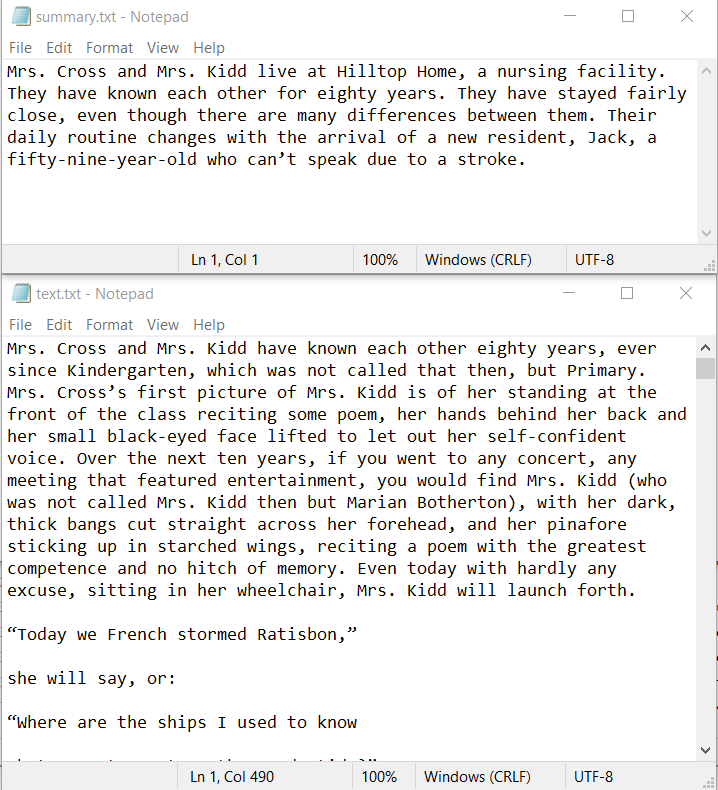
\includegraphics[scale=0.5]{short_story_data.png}
  \caption{Short story dataset sample}
  \label{fig:Short story Dataset Sample}
\end{figure}

\subsection{Problem Definition}
Suppose $s_0$ is the Begining of Sequence (BOS) token, $S_{doc} = \{s_1^d, s_2^d, ..., s_D^d\}$ is the original document, $S_{ref} = \{s_1^r, s_2^r, ..., s_R^r\}$ is the corresponding human annotated summary, $S_{gen} = \{s_1^g, s_2^g, ..., s_G^g\}$ is the corresponding actor generated summary, $S_{doc-ref}=\{s_0, S_{doc}, S_{ref}\}$ is the prepended concatenation of $S_{doc}$ and $S_{ref}$, $S_{doc-gen}=\{s_0, S_{doc}, S_{gen}\}$ is the prepended concatenation of $S_{doc}$ and $S_{gen}$, $D_{doc-ref}=\{S_{doc-ref}^{(1)}, S_{doc-ref}^{(2)}, ..., S_{doc-ref}^{(N)}\}$ is the set of all $S_{doc-ref}$, and $D_{doc-gen}=\{S_{doc-gen}^{(1)}, S_{doc-gen}^{(2)}, ..., S_{doc-gen}^{(N)}\}$ is the set of all $S_{doc-gen}$. Label $S_{doc-gen}$ as $l_0$ and $S_{doc-ref}$ as $l_1$.

\subsection{Baseline Models}

We use two different pretrained models as baselines for comparison, BART language model finetuned on CNN/DM dataset and SemSim model. Notice that due to hardware limitation, we cannot follow the training configuration of the baseline BART model or the SemSim model. Compared to their configuration, the maximum number of tokens per sample we use is smaller (BART allows samples as long as 2048 tokens, SemSim 1792, ours 1024), which means we have to truncate longer samples. There will be inevitable information loss due to this truncation, so when evaluating on the CNN/DM dataset, we would report two scores each for the BART and SemSim baseline models, one as reported accordingly in the original paper, and another one truncated to the same token size 1024 tokens per sample as ours.

\subsubsection{BART}

BART is a denoising autoencoder for pretraining sequence-to-sequence models. Originally, BART is trained by first corrupting text with an
arbitrary noising function, and then learning a model to reverse this procedure and reconstruct the original text. In this way, BART
can effectively learn contextual representations. The structure of BART consists of two parts, a generalized BERT\cite{devlin2018bert} bidirectional encoder, and an auto-regressive decoder following the settings of GPT\cite{radford2018improving}. The pre-trained BART model can be fine-tuned to various tasks such as translation, classification, and summarization. When fine-tuned for summarization task, the model will predict a probability distribution of token $s_t^g$ given input document $S_{doc}$ and previous tokens ${s_1^g, s_2^g, ..., s_{t-1}^g}$, $p(s_t^g|S_{doc}, s_1^g, s_2^g, ..., s_{t-1}^g)$, at time step $t$. Then the model is trained using maximum-likelihood loss $L_{ml}$
\begin{equation}
    L_{ml} = -\sum_{t=1}^m \log p(s_t^g|S_{doc}, s_1^g, s_2^g, ..., s_{t-1}^g)
\end{equation}

\subsubsection{SemSim}

This model consits of a language model $\Phi_{LM}$ which generates $S_{gen}$ given $S_{doc}$, and a pretrained rewarder $\Phi_{R}$ is used to output rewards given $S_{ref}$ and $S_{gen}$. During the training process, $\Phi_{R}$ will be fixed and $\Phi_{LM}$ will be trained using maximum-likelihood loss and the reward from $\Phi_{R}$. The authors use this structure so that the language model $\Phi_{LM}$ can learn from the semantic similarity between $S_{ref}$ and $S_{gen}$. To do so, another pre-trained LM, such as BERT, is used to encode each token of the input sequence as a dense vector, $e_{ref}=LM(S_{ref}), e_{gen}=LM(S_{gen})$, and then computes the semantic similarity loss as

\begin{equation}
    L_{reward} = -\Phi_{R}([e_{ref}; e_{gen}])
\end{equation}

The loss used to train the model will be the combination of maximum-likelihood loss $L_{ml}$ and semantic similarity loss

\begin{equation}
    L_{SemSim} = L_{ml} + wL_{reward}
\end{equation}

where $w$ acts as weight and is a hyperparameter to set. The language model $\Phi_{LM}$ used is a pre-trained BART model fine-tuned on CNN/DM dataset.

\subsection{Model}
We plan to use the actor-critic structure, which is first introduced in the context of reinforcement learning\cite{konda2000actor}, to develop a network for text summarization. There are two models in the actor-critic structure, namely the actor and the critic, where the actor will learn to complete a task, in other words perform actions given inputs, and the critic model will learn to judge how well the actor performs given inputs, actor's actions, and feedbacks from the environments if available.

Our actor-critic text summarization network consists of two parts, an actor network and a critic network. We'll use pre-trained BART language model for both networks. The actor network learn to produce a summary for the input document, and the critic network will learn to classify between the actor generated summary and the human annotated summary. The actor and critic networks will be trained alternately. Denote the actor network as $\Phi_{actor}$ and the critic network as $\Phi_{critic}$.

For critic network, the input will be randomly chosen from $D_{doc-ref}\cup D_{doc-gen}$. Denote the input as $S_{cirtic}$, then the output will be $\Phi_{critic}(S_{cirtic})=P(l_0|S_{cirtic})$. The critic network will be trained with cross entropy loss $L_{CE}$.

For actor network, the input will be $S_{doc}$, the output will be $\Phi_{actor}(S_{doc})=S_{gen}$, and the loss will be

\begin{equation}
    L_{actor} = L_{ml} + w\Phi_{critic}(\{s_0, S_{doc}, S_{gen}\})
\end{equation}
where $w$ acts as weight and is a hyperparameter we set.

The network structure is shown in Figure \ref{fig:network structure}. 

\begin{figure*}[h!]
    \centering
    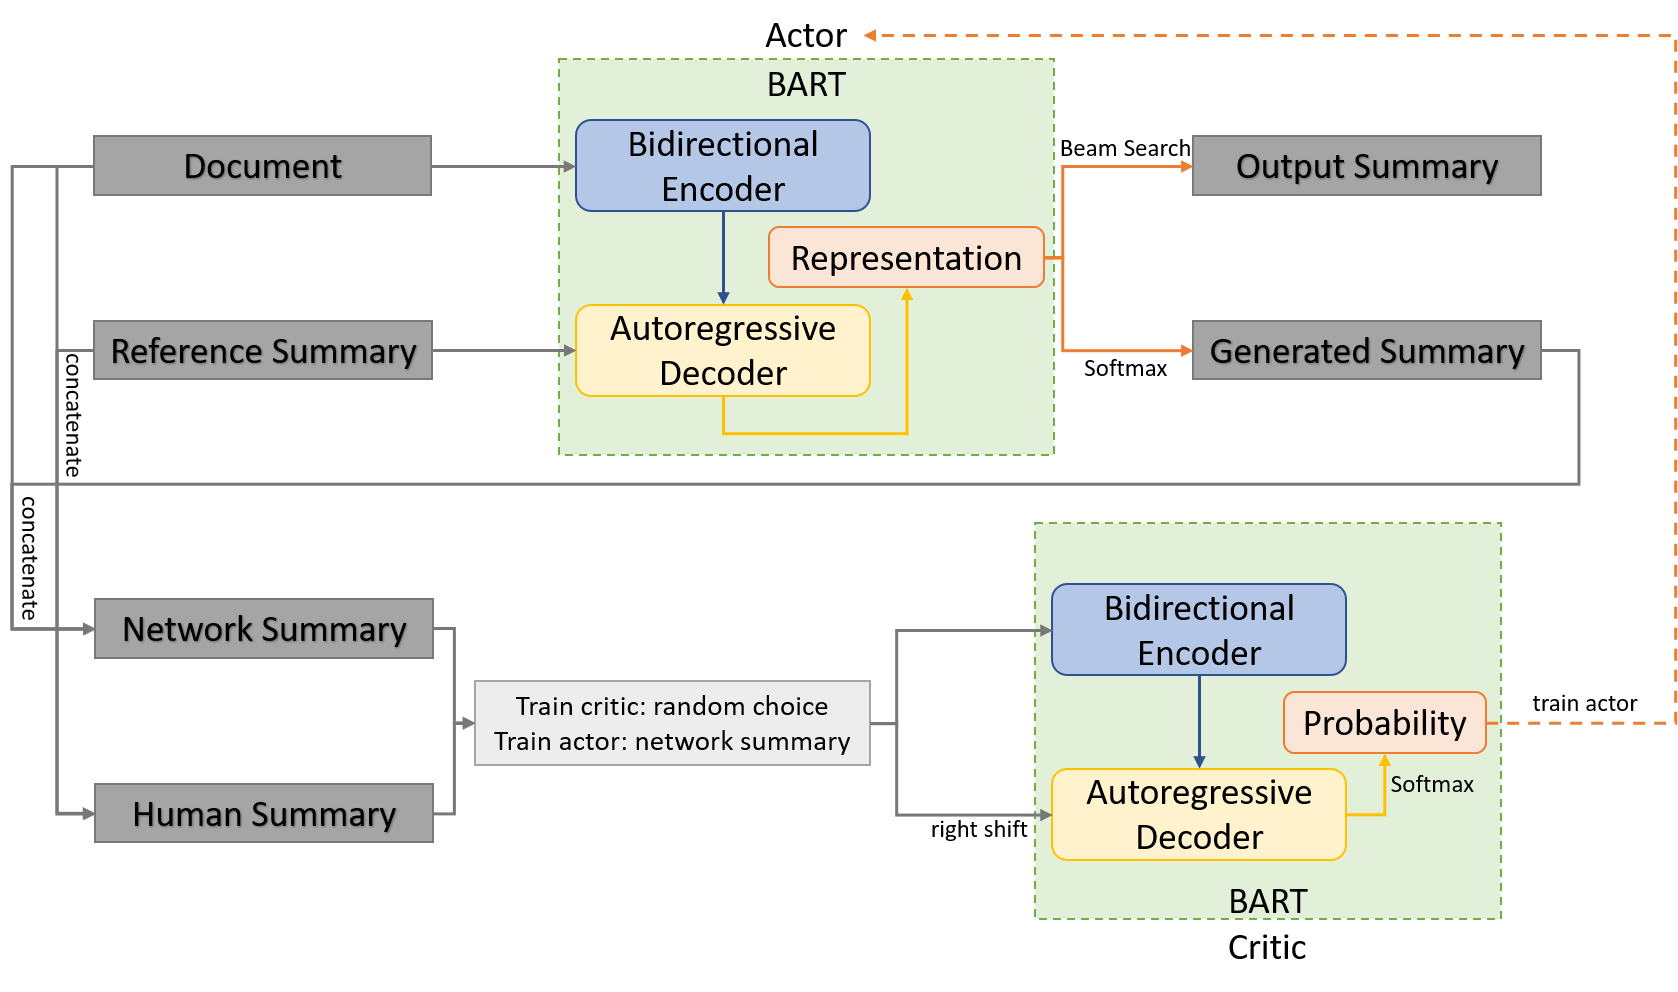
\includegraphics[width=\textwidth]{network structure.png}
    \caption{Our Actor-Critic Text Summarization Network Structure}
    \label{fig:network structure}
\end{figure*}

In our model, the actor $\Phi_{actor}$ and the critic $\Phi_{critic}$ will be trained to compete with each other. Generally, the actor will learn from the difference between its generated summaries and the reference human annotated summaries, so that the generated summaries will be more similar to the reference ones and the critic will be fooled; meanwhile the critic will also learn from the difference between actor generated summaries and the reference human annotated summaries so that it can better classify the two. $\Phi_{actor}$ and $\Phi_{critic}$ will be updated in an alternating manner. During the training process, we first fix $\Phi_{actor}$ and update $\Phi_{critic}$ for $N_{critic}$ times so the updated $\Phi_{critic}'$ can classify generated summaries from the current $\Phi_{actor}$ and reference summaries with a high accuracy, then we update $\Phi_{actor}$ for $N_{actor}$ times so the updated $\Phi_{actor}'$ can generate summaries that the current $\Phi_{critic}'$ has a hard time classifying. We call this one training loop, and the whole training process consists of $N_{loop}$ training loops. $N_{actor}$, $N_{critic}$, and $N_{loop}$ are hyperparameters we set. We'll repeat until the actor network can generate high quality summaries. The evaluation metrics for $\Phi_{actor}$ is ROUGE\cite{lin-2004-rouge} scores, and the evaluation metrics for $\Phi_{critic}$ is classification accuracy.

For the critic network, we use pre-trianed BART language model finetuned on GLUE benchmark\cite{wang2018glue} MNLI task, and for the actor network, we use pre-trained BART language model finetuned on CNN/DM dataset. Therefore, we'll evaluate and test our model on CNN/DM dataset, the same as the pre-trained language model we use so that we'll have a better comparison.

\section{Result}
\label{result}
\subsection{Primary Experiment Setup}
\label{setup}

The primary experiment we conduct is to train and evaluate our own actor-critic text summarization model on the standard dataset CNN/DM. The CNN/DM dataset contains online news articles which have 781 tokens on average and their corresponding multi-sentence summaries which have 3.75 sentences and 56 tokens on average. We use the same non-anonymized version of the data as used in \cite{see2017get, yoon2020learning}, which has 287,226 training pairs, 13,368 validation pairs and 11,490 test pairs.

We run all our experiments on a Google Cloud Platform instance with 1 16GB NVIDIA Tesla T4 GPU, 4v Intel Skylake structure CPU, and 20 GB RAM. When training our own model, we used the memory efficient 16-bit float point (fp16) version of Adam optimizer and a polynomial learning rate scheduler that decay the learning rate by a given factor once every update for both the actor and the critic networks due to hardware limitations. The actor and critic networks  The critic is trained for 2048 updates in the initial training loop and 512 updates in other loops with batch size 1, peak learning rate 5e-6, and learning rate decay factor $\frac{1}{13}$. It takes about 4 hours to train the critic for one loop because the critic has reached a pretty high accuracy of over 0.96, so we stop training in an early stage. The actor is trained for 6144 updates which is about 1.5 epochs in each training loop with batch size 64, peak learning rate 1e-5, and learning rate decay factor $\frac{1}{39}$. Weight for critic score is set to $\frac{100}{32}$. It takes about 48 hours to train the actor for one epoch and about 72 hours for one loop. The actual training time is longer because we periodically evaluate and save checkpoints during the training process. Since training for one loop takes a very long time, we cannot do a thorough hyper-parameter search. We only tried for a few sets of hyper-parameters, and the result reported below is trained with the reported hyper-parameters above for 2 loops and is the best one so far.


\subsection{Result Comparison}
\subsubsection{Evaluation Results}

We use the widely used ROUGE\cite{lin-2004-rouge} score, namely F-1 scores of ROUGE-1, ROUGE-2 and ROUGE-L \cite{paulus2017deep, see2017get, lewis2019bart} to evaluate our model and the baseline models on the test split of CNN/DM dataset. When evaluating the baseline models, we use the pre-trained weights provided by the corresponding authors. However, since the original baseline models BART and SemSim are trained with different maximum input size, which is 2048 for BART and 1792 for SemSim compared with 1024 for ours, and smaller maximum input size may affect the model performance, we adopted the pretrained weights for both baseline models to maximum input size 1024. After this adoption, there is significant drops in evaluation score for BART but not for SemSim, so we report two scores for BART, one before adoption, which is the same as reported in the original paper, and another one after adoption. The results are shown in Table \ref{tab:result}

\begin{table*}[h!]
    \centering
    \caption{Results on CNN/DM Dataset}
    \label{tab:result}
    \begin{tabular}{|l|c|c|c|}
    \hline
        model & ROUGE-1 & ROUGE-2 & ROUGE-L \\\hline
        \textbf{BART}(reported) & 44.16 & 21.28 & 40.90 \\\hline
        \textbf{BART}(baseline) & 43.99 & 21.07 & 40.82 \\\hline
        \textbf{SemSim} & 44.72 & 21.46 & 41.53 \\\hline
        \textbf{Ours} & 44.70 & 21.53 & 41.49 \\\hline
    \end{tabular}
    \subcaption{Automatic Evaluation Scores}
    \fbox{
    \begin{minipage}{\dimexpr\linewidth}\textbf{Original Text(truncated):} ..."The Price Is Right" encountered not host Drew Carey but another familiar face in charge of the proceedings. Instead, there was Bob Barker, who hosted the TV game show for 35 years before stepping down in 2007. Looking spry at 91, Barker handled the first price-guessing game of the show, the classic "Lucky Seven," before turning hosting duties over to Carey, who finished up...\\\hline\\
    \textbf{Reference Summary:} Bob Barker returned to host "The Price Is Right" on Wednesday. Barker, 91, had retired as host in 2007.\\\hline\\
    \textbf{BART:} Bob Barker returned to `` The Price Is Right '' for the first time in eight years . He hosted the show for 35 years before stepping down in 2007 . The 91-year-old did n't seem to miss a beat on the April 1 edition of the game show .\\\hline\\
    \textbf{SemSim:} Bob Barker returned to `` The Price Is Right '' for the first time in eight years . The 91-year-old host hosted the April 1 edition of the game show . He hosted the show for 35 years before stepping down in 2007 . Drew Carey finished up the show , which aired April 1 .\\\hline\\
    \textbf{Ours:} Bob Barker returned to `` The Price Is Right '' for the first time in eight years . The 91-year-old hosted the show for 35 years before stepping down in 2007 . Drew Carey finished up after Barker handled the first game of the show 's classic `` Lucky Seven ''
    \end{minipage}}
    \subcaption{Examples of Generated Summaries}
\end{table*}

\subsubsection{Result Analysis}

In the automatic evaluation, our model outperforms the baseline BART model by 1.71(3.89\%), 0.46(2.18\%), and 0.67(1.64\%) in ROUGE-1, ROUGE-2, and ROUGE-L scores respectively. However, our model only achieves a similar performance as the baseline SemSim model, with a -0.02(0.04\%), 0.07(0.33\%), and -0.04(0.10\%) difference in ROUGE-1, ROUGE-2, and ROUGE-L scores respectively. 

We think this is mainly because we haven't trained the actor to convergence. As shown in figure \ref{fig:loss}, both the total loss and the critic score are still showing clear sign of decreasing, which means the actor hasn't converged yet. The critic score is still high ($>0.7$) when we stop training, which means the actor hasn't learned to fool the critic. Therefore, if we keep training for more training loops, it's possible for the model to achieve better performance. Modifying the training strategy may also has better result. As can be seen in figure \ref{fig:loss}, both the total loss and the critic score decrease fast during the early stage of training but decrease much more slowly as the training goes on. Currently, we try to first train the actor long enough to fool the critic before switching to the next loop and start training the critic. It may be better to first train the actor for only a while until the actor gets a little better at fooling the critic, and then go ahead to train the critic. In this way, it's possible that the decreasing in loss remain fast throughout the training, so we can achieve better performance in equal or less time. Also, due to time limitation, we can only train the actor for about 3 epochs while the SemSim is reported to be trained for 6 epochs.

The hyper-parameters we use is not fully tuned, and the current critic network structure we use may be too good at classifying between the generated summaries and the reference summaries, so the critic score won't decrease much no matter how hard the current actor network tries. It may be better to switch to a different critic network.

\begin{figure}[h!]
    \centering
    \caption{Training Statistics Plot}
    \label{fig:loss}
    \begin{subfigure}{\linewidth}
    \centering
    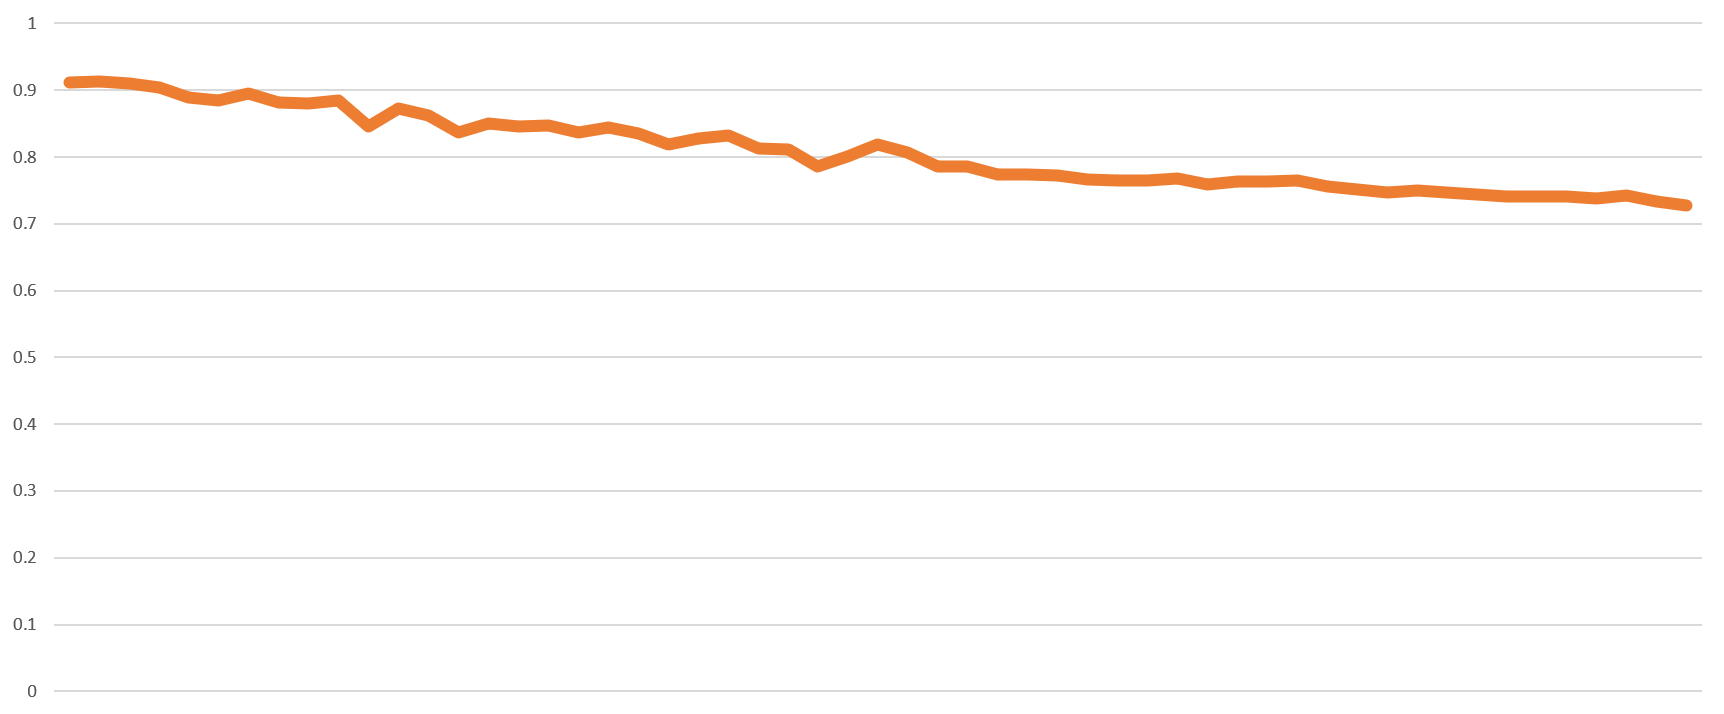
\includegraphics[width=\linewidth]{critic.png}
    \subcaption{Critic Score}
    \end{subfigure}
    \begin{subfigure}{\linewidth}
    \centering
    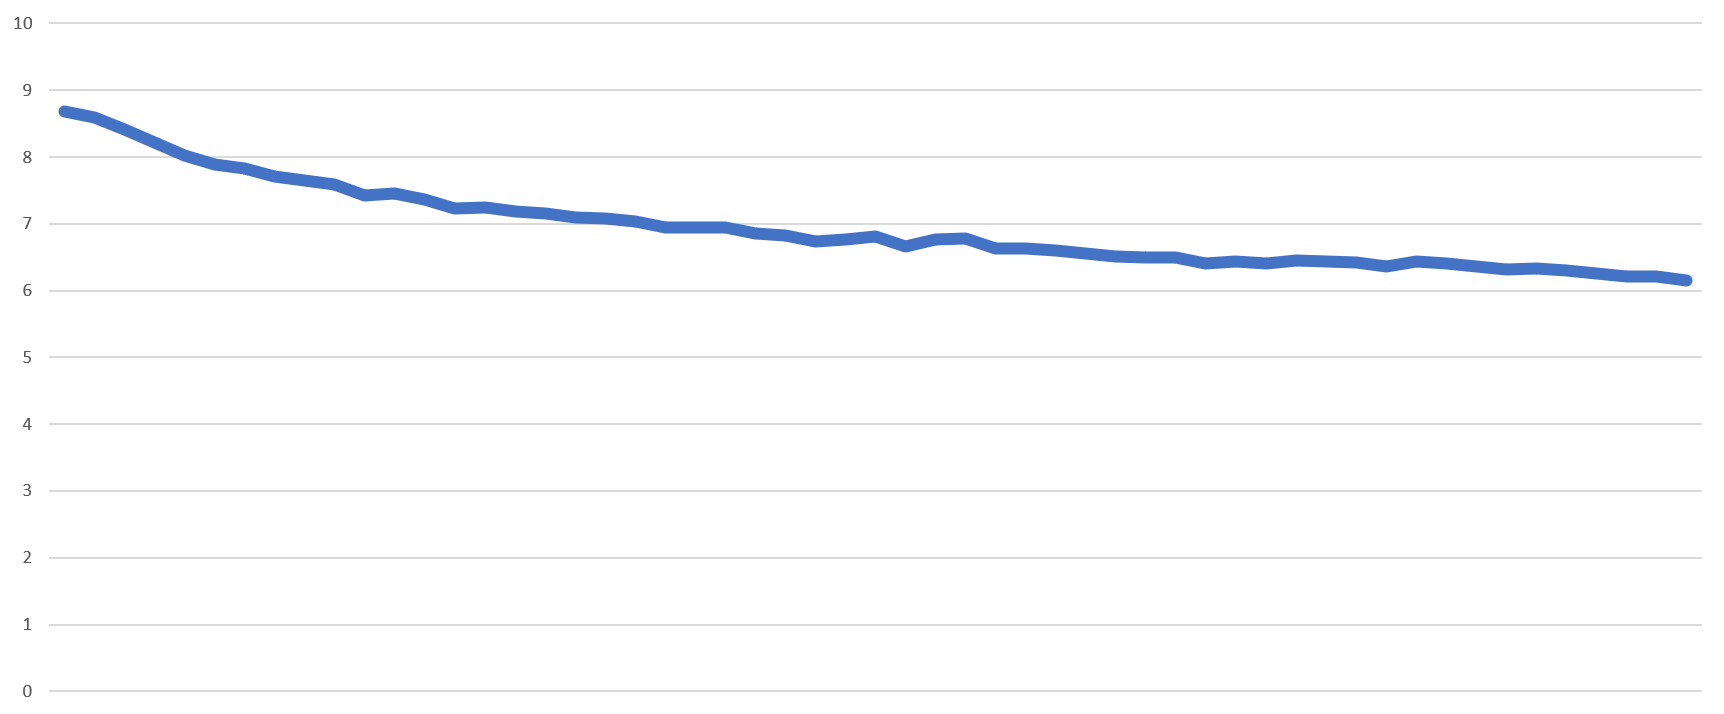
\includegraphics[width=\linewidth]{loss.png}
    \subcaption{Total Loss}
    \end{subfigure}
\end{figure}

Currently, the errors commonly seen in the generated summaries from our network including over emphasis on names of people or entities, such as shown in the table \ref{tab:result}, where the unimportant names "Drew Carey" and "Lucky Seven" is included; over sensitivity to numbers, such as shown in \ref{number}; and repentance of common tokens, such as shown in \ref{token}.

\begin{table*}[h!]
    \centering
    \caption{Examples of Some of the Common Errors}
    \fbox{
    \begin{minipage}{\dimexpr\linewidth}\textbf{Original Text (truncated):} ...The historic California drought hurts the rest of the union, too. That's because California is a breadbasket to the nation, growing more than a third of its vegetables and nearly two-thirds of its fruits and nuts. Here's why we should heed the ongoing drought in the most populous state, a slowly expanding natural disaster now in its fourth year that this week prompted Gov. Jerry Brown to announce a mandatory 25\% cutback in water consumption in all cities. In 2014, one expert predicted consumers would pay more for some groceries because of the California drought...\\\hline\\
    \textbf{Reference Summary:} Americans paid more for some fruits and vegetables last year because of the drought. Tourists will now have to ask for a glass of water at a California restaurant. Perhaps the only good thing is another "great" wine grape harvest last year.\\\hline\\
    \textbf{Ours:} California is a breadbasket to the nation , growing more than a third of its vegetables and nearly two-thirds of its fruits and nuts . Gov. Jerry Brown this week announced a mandatory 25\% cutback in water consumption in all cities . The drought is affecting other states in the West and Southwest as well .
    \end{minipage}}
    \subcaption{Over Sensitivity to Numbers}
    \label{number}
    \fbox{
    \begin{minipage}{\dimexpr\linewidth}\textbf{Original Text:} ...It's now classified as a tropical storm, according to the Philippine national weather service, which calls it a different name, Chedeng. It boasts steady winds of more than 70 mph (115 kph) and gusts up to 90 mph as of 5 p.m. (5 a.m. ET) Saturday. Still, that doesn't mean Maysak won't pack a wallop. Authorities took preemptive steps to keep people safe such as barring outdoor activities...\\\hline\\
    \textbf{Reference Summary:} Once a super typhoon, Maysak is now a tropical storm with 70 mph winds. It could still cause flooding, landslides and other problems in the Philippines.\\\hline\\
    \textbf{Ours:} NEW : Maysak is no longer classified as a super typhoon . NEW : It 's now a tropical storm . It boasts steady winds of more than 70 mph (115 kph) It 's expected to make landfall Sunday morning on the southeastern coast of Isabela province . Authorities take preemptive steps to keep people safe.
    \end{minipage}}
    \subcaption{Repeated Tokens}
    \label{token}
\end{table*}

\subsection{Experiments on CL-SciSumm Dataset and English Short Story Dataset}

We have run experiments on both the CL-SciSumm dataset and our own English short story dataset. For CL-SciSumm dataset, we used 848 samples as training set, 45 samples as validation set, and 20 samples as test set. For our own English short story dataset, we used 325 samples as training set, 41 samples as validation set, and 36 samples as test set. All the three models have been trained for 50 epochs on both datasets. The training setup for our dataset has been the same as described in section \ref{setup}. The setups for both baseline models have been in alignment with those used in corresponding original papers. In details, the optimizer is memory efficient fp16 version of Adam, the batch size is 32, learning rate 3e-5 with a polynomial decay at the rate of $\frac{1}{39}$, and maximum input tokens 1024. We run automatic evaluation with ROUGE score on the test splits. The evaluation results is shown in Table \ref{tab:exp}. We also include some examples on both dataset in Appendix \ref{sec:appendix}.

\begin{table}[h]
    \centering
    \caption{Results on CL-SciSumm Dataset and English Short Story Dataset}
    \label{tab:exp}
    \begin{tabular}{|l|c|c|c|}
    \hline
        model & ROUGE-1 & ROUGE-2 & ROUGE-L \\\hline
        \textbf{BART} & 38.15 & 14.04 & 25.31 \\\hline
        \textbf{SemSim} & 36.71 & 12.93 & 23.72 \\\hline
        \textbf{Ours} & 38.40 & 14.01 & 24.28 \\\hline
    \end{tabular}
    \subcaption{Evaluation Scores on CL-SciSumm Dataset}
    \begin{tabular}{|l|c|c|c|}
    \hline
        model & ROUGE-1 & ROUGE-2 & ROUGE-L \\\hline
        \textbf{BART} & 31.89 & 7.70 & 28.73 \\\hline
        \textbf{SemSim} & 31.42 & 7.73 & 28.03 \\\hline
        \textbf{Ours} & 31.24 & 7.85 & 28.90 \\\hline
    \end{tabular}
    \subcaption{Evaluation Scores on English Short Story Dataset}
\end{table}

Currently we are truncating the input to 1024 tokens, which will lose a large part of information because inputs in both datasets are much longer than this. We think this is the main reason why all three models have similar performance on the two datasets. Due to time limitation, we don't have the chance to test the two datasets with BERT representations as input instead of the tokens.

\subsection{Work Division}

Haoxin Ma is responsible for collecting half of the English short story dataset; implementing, training and evaluating our own actor-critic text summarization network and the baseline networks BART and SemSim; processing the CNN/DM dataset; running all the experiments; result analysis; and the presentation. Quanfei Zhang is responsible for collecting another half of the English short story dataset, data pre-process for CL-SciSumm dataset and our own English short story dataset, result analysis, and the presentation.

\section{Discussion}
\label{discuss}
\subsection{Conclusions}

In this project, we propose an actor-critic structure for text summarization. In our structure, there are two networks trained to compete with each other, the critic one trying to classify between the generated and reference summaries, and the actor one trying to generated summaries that can fool the critic. From the results of our project, we find learning text summarization from the difference between the reference and generated summaries by training two models adversarially can improve the quality of the generated summaries. Summaries generated by our structure tend to extract salient information while taking a different form and meaning from the reference one.

Compared with \cite{yoon2020learning}, we find that besides learning from the semantic similarity between the reference and generated summaries, it's also effective to learn from the difference between the two. While learning from semantic similarity encourage the generated summary to have similar ``meaning" as the reference one, learning from the difference appears to learning something more representative, as the summaries generated from our model have extracted the important information while not having similar meanings as the reference one compared to ones generated from \cite{yoon2020learning}.

\subsection{Future Works}

There are many possible directions to continue the work in this project. First, a better training strategy could be found to train both the networks because the current training loop strategy doesn't appear efficient enough. The current training loop is not the same as the common training strategy used for actor-critic structure in RL, where the actor and critic would be trained simultaneously based on the reward received from the environment. It may be possible to use a designed or learned reward function and train the actor-critic structure with another training strategy. Also, our actor and critic networks use the same pre-trained network as backbone, it may be possible to use different backbones.

For the data part, it's worth a try to use BERT or other language model to first generate representations for long documents in CL-SciSumm and our English short story dataset and try to train text summarization models with the representations as input instead of the tokens.

\bibliography{acl2020}
\bibliographystyle{acl_natbib}

\appendix
\onecolumn
\section{Appendices}
\label{sec:appendix}
\subsection{Example on CL-SciSumm Dataset}
    \fbox{
    \begin{minipage}{\dimexpr\linewidth}\textbf{Original Text(truncated):} ...What fundamentally distinguishes probabilistic generative parsers is how they compute p(r), and it is to that topic we turn next.The model assigns a probability to a parse by a top-down process of considering each constituent c in Ir and for each c first guessing the pre-terminal of c, t(c) (t for &quot;tag&quot;), then the lexical head of c, h(c), and then the expansion of c into further constituents e(c).Thus the probability of a parse is given by the equation where 1(c) is the label of c (e.g., whether it is a noun phrase (np), verb-phrase, etc.) and H (c) is the relevant history of c — information outside c that our probability model deems important in determining the probability in question.Much of the interesting work is determining what goes into H (c).Whenever it is clear to which constituent we are referring we omit the (c) in, e.g., h(c)...\\\hline\\
    \textbf{Reference Summary(truncated):} We present a new parser for parsing down to Penn tree-bank style parse trees that achieves 90.1\% average precision/recall for sentences of 40 and less, and for of length 100 and less when trained and tested on the previously established sections of the Wall Street Journal treebank...\\\hline\\
    \textbf{BART:} We present a new parser for parsing down to Penn tree-bank style parse trees that achieves 90.1 \% average precision/recall for sentences of length < 40 , and 89.5 \% for sentence length < 100 . This represents a 13 \% decrease in error rate over the best single-parser results on this corpus . Our parser is based upon a probabilistic generative model.That is , for all sentences s and all parses 7r , the parser assigns a probability p ( s , 7r ) = p ( r ) , the equality holding when we restrict consideration to 7r whose yield yield * is s .\\\hline\\
    \textbf{SemSim:} We present a new grammar for parsing down to Penn tree-bank style parse trees that achieves 90.1 \% average precision/recall for sentences of length < 40 , and 89.5 \% for sentences < 100 , when trained and tested on the previously established `` standard" ; sections of the Wall Street Journal tree - bank.This represents a 13 \% decrease in error rate over the best single-processor results on this corpus. Our Parser is based upon a probabilistic generative model.That is , for all sentences s and all parses 7r.\\\hline\\
    \textbf{Ours:} We present a new grammar for parsing down to Penn tree-bank style parse trees that achieves 90.1 \% average precision/recall for sentences of length < 40 , and 89.5 \% for sentence of length less than 100 . This represents a 13 \% decrease in error rate over the best single-processor results on this corpus . Our Parser is based upon a probabilistic generative model.That is , for all sentences s and all parses 7r , the parser assigns a probability p ( s , 7r ) = p ( r ) .
    \end{minipage}}

\subsection{Example on Short Story Dataset}

    \fbox{
    \begin{minipage}{\dimexpr\linewidth}\textbf{Original Text(truncated):} Miss Martha Meacham kept the little bakery on the corner (the one where you go up three steps, and the bell tinkles when you open the door). Miss Martha was forty, her bank-book showed a credit of two thousand dollars, and she possessed two false teeth and a sympathetic heart. Many people have married whose chances to do so were much inferior to Miss Martha's...\\\hline\\
    \textbf{Reference Summary:} Miss Martha is a forty-year-old woman who owns a small bakery. She has a regular customer, a middle-aged man who always buys two loaves of stale bread, never anything else. She takes an interest in him, and tries to find a way to get to know him.\\\hline\\
    \textbf{BART:} Miss Martha Meacham is a forty-year-old bakery owner with a credit of two thousand dollars and a sympathetic heart . She buys two loaves of stale bread from a middle-aged man every time he comes in . She suspects he 's an artist , but he does not show any interest in her wares . One day she finds a pound of fresh butter on the bottom of the counter , and uses it to make him a new batch .\\\hline\\
    \textbf{SemSim:} Miss Martha Meacham , a forty-year-old woman , runs a bakery . She has a credit of two thousand dollars and a sympathetic heart . She takes an interest in a customer , a middle-aged man , who buys lots of stale bread . She suspects he is an artist , but he denies this , saying his work is n't good enough . Miss Martha tries to help him out by giving him some fresh bread .\\\hline\\
    \textbf{Ours:} Miss Martha Meacham , a forty-year-old bakery owner , has a credit of two thousand dollars and a sympathetic heart . She buys two loaves of stale bread from a middle-aged man every time he comes in . She suspects he is an artist , but he does not seem to recognize her suspicions . One day she is inspired to buy a pound of fresh butter from the bakery 's dairyman .
    \end{minipage}}

% Appendices are material that can be read, and include lemmas, formulas, proofs, and tables that are not critical to the reading and understanding of the paper. 
% Appendices should be \textbf{uploaded as supplementary material} when submitting the paper for review.
% Upon acceptance, the appendices come after the references, as shown here.

% \paragraph{\LaTeX-specific details:}
% Use {\small\verb|\appendix|} before any appendix section to switch the section numbering over to letters.


% \section{Supplemental Material}
% \label{sec:supplemental}
% Submissions may include non-readable supplementary material used in the work and described in the paper.
% Any accompanying software and/or data should include licenses and documentation of research review as appropriate.
% Supplementary material may report preprocessing decisions, model parameters, and other details necessary for the replication of the experiments reported in the paper.
% Seemingly small preprocessing decisions can sometimes make a large difference in performance, so it is crucial to record such decisions to precisely characterize state-of-the-art methods. 

% Nonetheless, supplementary material should be supplementary (rather than central) to the paper.
% \textbf{Submissions that misuse the supplementary material may be rejected without review.}
% Supplementary material may include explanations or details of proofs or derivations that do not fit into the paper, lists of
% features or feature templates, sample inputs and outputs for a system, pseudo-code or source code, and data.
% (Source code and data should be separate uploads, rather than part of the paper).

% The paper should not rely on the supplementary material: while the paper may refer to and cite the supplementary material and the supplementary material will be available to the reviewers, they will not be asked to review the supplementary material.

\end{document}
